\documentclass[11pt,a4paper]{article}

\usepackage[utf8]{inputenc}
\usepackage[T1]{fontenc}
\usepackage[margin=1in]{geometry}
\usepackage{booktabs}
\usepackage{graphicx}
\usepackage{amsmath}
\usepackage[round]{natbib}
\usepackage{hyperref}
\hypersetup{colorlinks=true,linkcolor=blue,citecolor=blue,urlcolor=blue}

\title{A Common Electrical-Energy Basis for Comparing Lunar Oxygen and Propellant Production Routes}
\author{Walter Kueffer}
\date{Draft manuscript, version 0.1 (2026-05-30)}

\begin{document}

\maketitle

\begin{center}
Code, data, and all figures are reproducible from the open-source model at\\
\url{https://github.com/dubthree/lunar-propellant-energy-model}.
\end{center}

\begin{abstract}
Lunar in-situ propellant production is widely proposed as the key to affordable
cislunar transport, yet the basic engineering question (which oxygen-extraction route
costs the least \emph{energy} per kilogram of product) is hard to answer from the
literature, because published figures are reported on incompatible bases: hydrogen
reduction as electrical energy, carbothermal reduction as thermal energy, and molten
regolith electrolysis (MRE) with no published figure at all. Prior work compares subsets
(\citet{taylor1993} reviewed $\sim$20 processes; \citet{leger2025} modeled several on a
common basis), but no published comparison places all five of these routes, including the
thermally-reported carbothermal route and the two electrolysis routes that lack any
published energy figure, on a single electrical-equivalent basis with paired uncertainty
propagation. We present a small, open, uncertainty-quantified model that places five
routes (hydrogen reduction, carbothermal reduction, MRE, molten-salt electrolysis, and
polar water-ice mining) on one electrical-equivalent kWh/kg O$_2$ basis under a single
explicit system boundary, with Monte-Carlo propagation of literature parameter ranges.
We check the framework against the one route with a clean published electrical figure
(hydrogen reduction, \citet{leger2025}, 24.3 $\pm$ 5.8 kWh/kg LOX): our nominal estimate
(24.6) lands within $\sim$1\% of Leger's central value, though our Monte-Carlo
distribution is centered somewhat lower (median $\sim$21), so we report this as
substantial interval overlap between two independent estimates rather than a point match.
We add historical and terrestrial cross-checks for MRE (\citealt{carr1963}, as reported
by \citealt{schreiner2016sizing}; terrestrial molten-oxide electrolysis), noting these
span different system boundaries. Using a paired Monte Carlo that shares common parameters
across routes, we report dominance probabilities rather than overlapping error bars.
Three findings emerge: (1) carbothermal reduction is the most likely lowest-energy route
(cheapest in 58\% of paired trials; it beats hydrogen reduction $\sim$100\% and MRE
$\sim$90\% of the time but only $\sim$75\% versus molten-salt and the water route),
visible only once routes share a common basis, though carbothermal is itself one of the
routes without an independent energy anchor; (2) in 99\% of trials the most
energy-intensive route is either hydrogen reduction (51\%) or MRE (48\%), and MRE's
reputation as low-energy does not survive a realistic full-cell voltage; (3) the polar
water route, though mid-pack per kg O$_2$, is the only route that yields a complete
LOX+LH$_2$ propellant. A sensitivity analysis identifies the single highest-value
measurement for each route. We translate energy into required surface power and landed
fission-plant mass, and outline two companion analyses on reusing co-located compute
waste heat.
\end{abstract}

\section{Introduction}

The case for lunar propellant rests on energy: every process that turns regolith or
polar ice into liquid oxygen (and ideally liquid hydrogen) is energy-intensive, and
surface power is the binding constraint on any near-term architecture. Yet the
comparison that should drive route selection has never been made on equal footing.
Three incompatibilities recur in the literature:

\begin{enumerate}
  \item \textbf{Thermal vs electrical energy are conflated.} Carbothermal reduction is
    reported as delivered thermal energy or ``g O$_2$/kWh thermal''; hydrogen reduction
    is reported as electrical kWh/kg. On the Moon both ultimately draw on the same
    scarce electrical supply, but they are not interchangeable at face value.
  \item \textbf{System boundaries differ.} Some figures include excavation,
    beneficiation, and liquefaction; others count only the reactor.
  \item \textbf{Two routes have no published figure at all.} Molten regolith
    electrolysis and molten-salt electrolysis are described qualitatively; their energy
    cost is asserted, not quantified.
\end{enumerate}

The consequence is that capital allocation, power-plant sizing, and architecture choice
rest on a comparison that does not exist. This is a modeling gap, not a hardware gap,
which is precisely why it can be closed now, cheaply, and reproducibly. We build that
comparison and quantify its uncertainty.

\section{Methods}

\subsection{Functional unit and system boundary}

We compute the \textbf{electrical-equivalent energy in kWh per kg of O$_2$ delivered to
cryogenic storage}, and additionally report kWh per kg of total propellant for the one
route that co-produces hydrogen. The system boundary is a fixed sequence of stages;
every route enables a subset, using the same stage sub-models, so all differences
between routes arise from parameters rather than inconsistent accounting:

\begin{quote}
excavation/acquisition $\rightarrow$ beneficiation $\rightarrow$ heating (sensible, plus
fusion for melt routes) $\rightarrow$ reaction (reduction enthalpy or Faradaic
electrolysis) $\rightarrow$ product cleanup $\rightarrow$ water electrolysis (where the
route produces H$_2$O) $\rightarrow$ gas compression $\rightarrow$ liquefaction (LOX
always; LH$_2$ where hydrogen is retained).
\end{quote}

\subsection{Thermal-to-electrical conversion}

To compare a thermally-reported route against electrically-reported ones, all thermal
demand is converted to electrical-equivalent through an explicit electric-to-thermal
efficiency parameter (resistive heating, nominal 0.90). This single, visible knob is
what makes the comparison honest; a solar-thermal heating pathway would be a separate
sensitivity, not the baseline.

\subsection{Uncertainty propagation}

Every uncertain input is a triangular \texttt{(low, nominal, high)} distribution sourced
from the literature (the full parameter table, with a citation on every value, is in
\texttt{params.py}). A 20,000-trial Monte Carlo propagates these to a 90\% interval per
route. We propagate stated literature ranges, not assumed Gaussian measurement error.
The electrolysis cell voltage and current efficiency of the electrochemical routes are
sampled with a physical anti-correlation (a shared operating-severity latent: higher
current density raises voltage and lowers efficiency together), avoiding unphysical
parameter corners.

\subsection{Ranking by paired Monte Carlo}

Reading a ranking from five marginal error bars is a statistical error, because the
routes share parameters (regolith specific heat, heat recuperation, electrolysis
efficiency, liquefaction) that must take the same value in any given world. We therefore
run a paired Monte Carlo: one shared parameter draw per trial across all routes,
evaluated trial by trial, so we can report P(route A cheaper than route B) and P(route
is cheapest / worst).

\section{Validation}

\subsection{Hydrogen reduction against Leger 2025 (and a second anchor)}

Hydrogen reduction is the only route with a clean published electrical figure: 24.3
$\pm$ 5.8 kWh/kg LOX, with the reduction step $\sim$55\% and water electrolysis
$\sim$38\% of the total \citep{leger2025}. We built our estimate bottom-up from first
principles and independent parameters; the largest tunable term (water-electrolysis
efficiency) is set from an independent SOEC source \citep{hauch2020,iea2019hydrogen},
not from Leger's implied value.

\begin{itemize}
  \item Nominal point estimate: \textbf{24.6 kWh/kg LOX}, within $\sim$1\% of Leger's
    central value and inside his 1-sigma interval [18.5, 30.1].
  \item The Monte-Carlo distribution is centered lower (median $\sim$21, mean $\sim$22):
    Leger's value sits near our 85th percentile, not our center. We therefore report
    agreement as substantial \textbf{interval overlap} between two independent estimates,
    not as a point match; the nominal coincidence to $\sim$1\% should not be over-read.
  \item Stage shares match: heating + reaction $\sim$65\% (Leger $\sim$55\%); water
    electrolysis $\sim$30\% (Leger $\sim$38\%).
  \item A second cross-check: \citet{taylor1993} place the route at $\sim$26 kWh/kg LOX
    (cross-technology range 18--35).
  \item Because the model omits several one-signed terms (Section~\ref{sec:limitations})
    that would raise totals, the nominal agreement with Leger and the lower distribution
    center are both consistent with the two estimates sharing a partial system boundary;
    we do not claim the absolute level is converged.
\end{itemize}

\subsection{MRE against Carr 1963 and terrestrial molten-oxide electrolysis}

MRE began as a pure first-principles estimate (nominal 18.5, median $\sim$21, 90\% CI
[12.9, 31.5]). Because it has no published electrical figure, we cross-check it against
three sources that unavoidably use \emph{different system boundaries}, so the agreement
is weak and bounding rather than a clean anchor: \citet{carr1963}, as reported
secondarily by \citet{schreiner2016sizing}, gives $\sim$26.4 kWh/kg O$_2$ for lunar MRE;
terrestrial molten-oxide electrolysis of iron runs $\sim$3.7--4.0 MWh/t metal, i.e.
$\sim$9 kWh/kg O$_2$, a well-insulated lower bound for a different chemistry
\citep{allanore2015}; and NASA reactor-sizing models place \emph{whole-system} figures
(including Joule heating and duty cycle, which our standalone-reactor boundary excludes)
at $\sim$50--120 kWh/kg O$_2$ \citep{schreiner2016sizing}. Our estimate falls between
these, which given their $\sim$9--120 spread is corroboration only in a loose sense. We
did, however, correct the oxide-melt current efficiency to match \emph{measured}
regolith-surrogate data (70--90\%, Ir anodes \citealp{allanore2015}) rather than an
optimistic assumption, a change that lowered MRE's estimate against the prior narrative.

These are the project's falsifiable tests (\texttt{tests/test\_validation.py}). Only
hydrogen reduction has a like-for-like published electrical figure; the others are
first-principles estimates reported with wide intervals and as probabilities, not point
claims.

\section{Results}

\begin{table}[ht]
  \centering
  \caption{Electrical-equivalent energy per route (20,000 trials).}
  \begin{tabular}{llrlr}
    \toprule
    Route & Yields & kWh/kg O$_2$ (nominal) & 90\% CI & kWh/kg propellant \\
    \midrule
    Carbothermal (CH$_4$)         & LOX       & 13.4 & 12.3--15.5 & 13.4 \\
    PSR water mining              & LOX+LH$_2$ & 14.4 & 12.8--17.3 & \textbf{12.8} \\
    Molten-salt (FFC)             & LOX       & 15.3 & 12.2--21.6 & 15.3 \\
    Molten regolith electrolysis  & LOX       & 18.5 (median 21) & 12.9--31.5 & 18.5 \\
    H$_2$ reduction (ilmenite)    & LOX       & 24.6 (median 21) & 16.9--27.6 & 24.6 \\
    \bottomrule
  \end{tabular}
  \label{tab:routes}
\end{table}

The single value is the deterministic nominal (all parameters at their cited value). For
the right-skewed electrochemical routes the Monte-Carlo \emph{median} differs materially:
notably MRE and hydrogen reduction share a median of $\sim$21 kWh/kg O$_2$, so although
their nominals differ (18.5 vs 24.6) they are statistically tied as the two most
intensive routes (Table~\ref{tab:dominance}). For plant sizing, prefer the median and the
interval over the nominal.

\begin{figure}[ht]
  \centering
  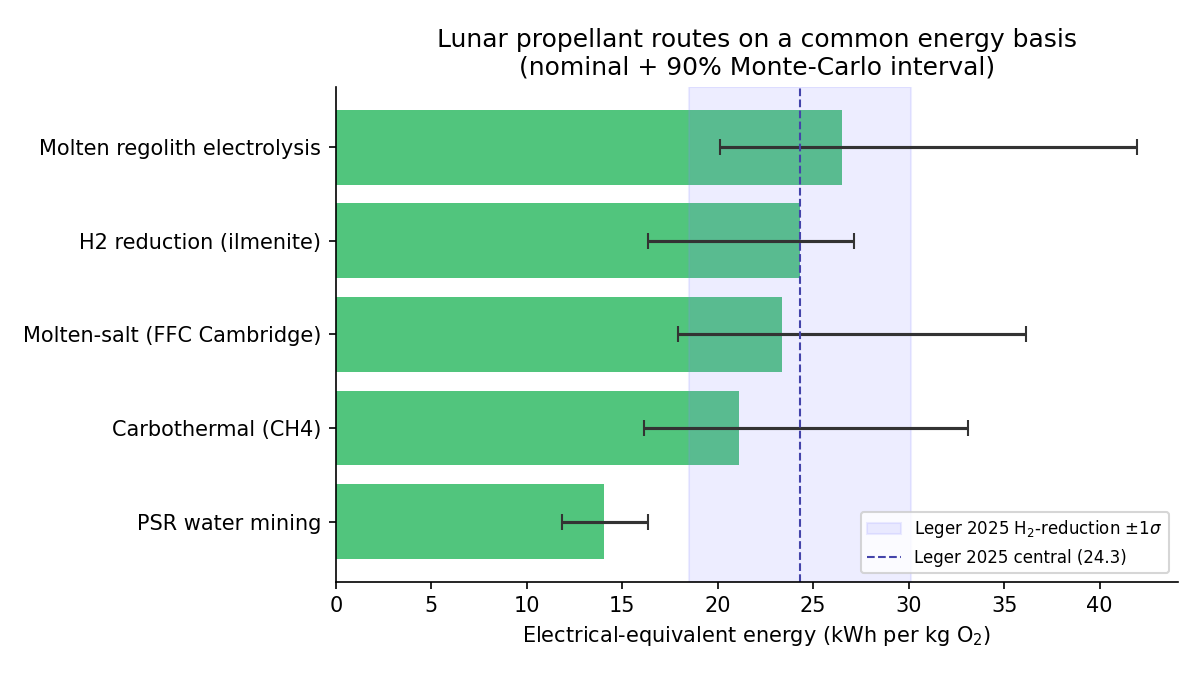
\includegraphics[width=0.85\textwidth]{../results/fig-routes.png}
  \caption{The five routes on a common electrical-energy basis (nominal + 90\%
  Monte-Carlo interval); the shaded band is Leger 2025's 1-sigma for hydrogen
  reduction.}
  \label{fig:routes}
\end{figure}

\begin{table}[ht]
  \centering
  \caption{Paired-Monte-Carlo dominance.}
  \begin{tabular}{lrr}
    \toprule
    Route & P(cheapest) & P(worst) \\
    \midrule
    Carbothermal (CH$_4$)        & 0.58 & 0.00 \\
    Molten-salt (FFC)            & 0.22 & 0.00 \\
    PSR water mining             & 0.19 & 0.00 \\
    Molten regolith electrolysis & 0.02 & 0.48 \\
    H$_2$ reduction (ilmenite)   & 0.00 & 0.51 \\
    \bottomrule
  \end{tabular}
  \label{tab:dominance}
\end{table}

Carbothermal beats hydrogen reduction in 100\% of paired trials and MRE in $\sim$90\%.
Molten-salt and the water route trade second place and are not separable.

\section{Sensitivity analysis}
\label{sec:sensitivity}

A one-at-a-time tornado analysis (each parameter swept low-to-high, all others nominal;
\texttt{python -m lpem --sensitivity <route>}) identifies the dominant uncertainty for
each route and, with it, the single highest-value measurement:

\begin{table}[ht]
  \centering
  \caption{Dominant sensitivity driver per route.}
  \begin{tabular}{lll}
    \toprule
    Route & Dominant driver (swing, kWh/kg O$_2$) & Next \\
    \midrule
    H$_2$ reduction & O$_2$ yield (13.3) & heat recuperation (9.1), cp (5.3) \\
    Carbothermal & reaction enthalpy (3.5) & yield (1.8), electrolysis eff (1.7); flat tornado \\
    MRE & \textbf{cell voltage (15.9)} & yield (3.8), current efficiency (3.7) \\
    Molten-salt & current efficiency (5.6) & cell voltage (4.5) \\
    PSR water & \textbf{LH$_2$ liquefaction (6.0)} & electrolysis eff (1.7), ice grade (1.0) \\
    \bottomrule
  \end{tabular}
  \label{tab:sensitivity}
\end{table}

Two practical conclusions: MRE's entire energy verdict hinges on one unmeasured number,
its full-cell decomposition voltage; pinning it with reactor data is the highest-value
measurement this model identifies. The water route's verdict hinges on small-scale
LH$_2$ liquefaction performance. The route ranking itself is robust: carbothermal's lead
and the hydrogen-reduction/MRE disadvantage survive across the parameter ranges
(Section~\ref{sec:findings}).

\section{Findings}
\label{sec:findings}

\textbf{Finding 1: Carbothermal is the most likely lowest-energy route, visible only on a
common basis.} Cheapest in 58\% of paired trials; it beats hydrogen reduction in
$\sim$100\% of trials and MRE in $\sim$90\%, but only $\sim$75\% versus molten-salt and
the water route, so it is the most likely winner, not a certain one. Its high O$_2$ yield
($>$20 wt\%) means it heats only $\sim$5 kg of regolith per kg O$_2$, versus $\sim$50 kg
for hydrogen reduction. Recast from its usual thermal basis onto the common electrical
basis, it comes out ahead, a comparison not previously made. One caveat we state plainly:
unlike hydrogen reduction and MRE, carbothermal has no independent published energy
figure, and its lead rests on an assumed high yield and a first-principles reaction
enthalpy that includes a Sabatier exotherm credit. Its lead is robust to its \emph{own}
parameters (flat tornado, Section~\ref{sec:sensitivity}) but is model-internal pending a
measured electrical figure.

\textbf{Finding 2: Hydrogen reduction and MRE are the two most energy-intensive, and
MRE's ``low energy'' reputation does not survive a realistic cell voltage.} On the
Monte-Carlo median they are tied ($\sim$21 kWh/kg O$_2$ each) and one of the two is the
worst route in 99\% of trials (hydrogen reduction 51\%, MRE 48\%). Hydrogen reduction
pays to heat $\sim$50 kg regolith per kg O$_2$ at low ilmenite yield plus a separate
electrolysis step; it is reliably poor. MRE is the high-variance one (median $\sim$21, CI
[12.9, 31.5]): its Faradaic term depends on the full decomposition voltage ($\sim$3.5 V
including overpotential and ohmic drop), not the $\sim$1.7 V thermodynamic floor, and not
the 16--34 V Joule-\emph{heating} voltages sometimes quoted from concept papers. With
measured current efficiency, MRE is the single worst route whenever its cell voltage runs
high.

\textbf{Finding 3: Per-kg-O$_2$ scoring understates the only full-propellant route.}
Polar water mining is the only route that co-produces usable hydrogen, so it alone
yields a complete LOX+LH$_2$ propellant rather than LOX with fuel still shipped from
Earth. It is mid-pack per kg O$_2$ (14.4) but its value is closing the hydrogen loop,
not lowest energy; the apparent per-propellant edge (12.8) is within uncertainty and
excludes small-scale LH$_2$ liquefaction and zero-boil-off storage.

\section{From energy to power plant and landed mass}

Energy matters through what it costs to supply. Converting kWh/kg into continuous
surface power and the landed mass of the fission-surface-power (FSP) system it implies
(\texttt{lpem.arch}), even a modest 50 t O$_2$/yr plant requires $\sim$85--156 kWe,
comparable to NASA's 40-kWe FSP concept \citep{oleson2022fsp} scaled up (and roughly one
to $\sim$1.6 units of the later 100-kWe FY2030 target). Route choice swings landed
power-system mass by $\sim$16 t (carbothermal $\sim$19 t vs hydrogen reduction $\sim$35 t)
for the same oxygen output. The direction is robust; the magnitude scales with the FSP
specific mass and assumes an all-fission architecture (a solar-plus-storage plant would
be dominated by night-survival storage mass, not modeled here).

\section{Companion analyses (compute waste-heat integration)}

Two companion analyses, kept modular, examine reusing co-located compute waste heat:

\begin{itemize}
  \item \textbf{Low-grade thermal offset} (\texttt{WASTE-HEAT-OFFSET.md}). By the Second
    Law, compute waste heat ($\sim$330 K) can supply only low-grade ISRU demand. At the
    nominal 350 K reject temperature, comfortably above the $\sim$273 K sublimation
    target, it can in principle cover the water route's full thermal-mining term
    ($\sim$2.1 kWh/kg O$_2$, $\sim$14\% of the route; Figure~\ref{fig:wasteheat}); this
    offset falls off sharply and excludes the sublimation enthalpy if compute rejects
    below $\sim$273 K. It cannot supply high-grade reduction/electrolysis heat at all.

  \item \textbf{PSR co-location} (\texttt{PSR-COLOCATION.md}). A permanently shadowed
    region is both a cryogenic radiative sink for compute and the location of the water
    resource. Under an explicit radiator energy balance, PSR siting saves a median
    $\sim$46 t of radiator mass per MW of compute (nominal 51; 90\% CI $\sim$11--290, the
    wide upper tail reflecting and heuristically capping sunlit cases that cannot reject
    at all; Figure~\ref{fig:radiator}), and in $\sim$18\% of sampled conditions a sunlit
    330 K radiator cannot reject at 330 K without active cooling. The heat cascade itself
    is a modest bonus (saves $\sim$2.7 t reactor for the reference plant, break-even
    enabling probability $\sim$38\%); co-location is justified by the compute siting
    economics, not the cascade.
\end{itemize}

\begin{figure}[ht]
  \centering
  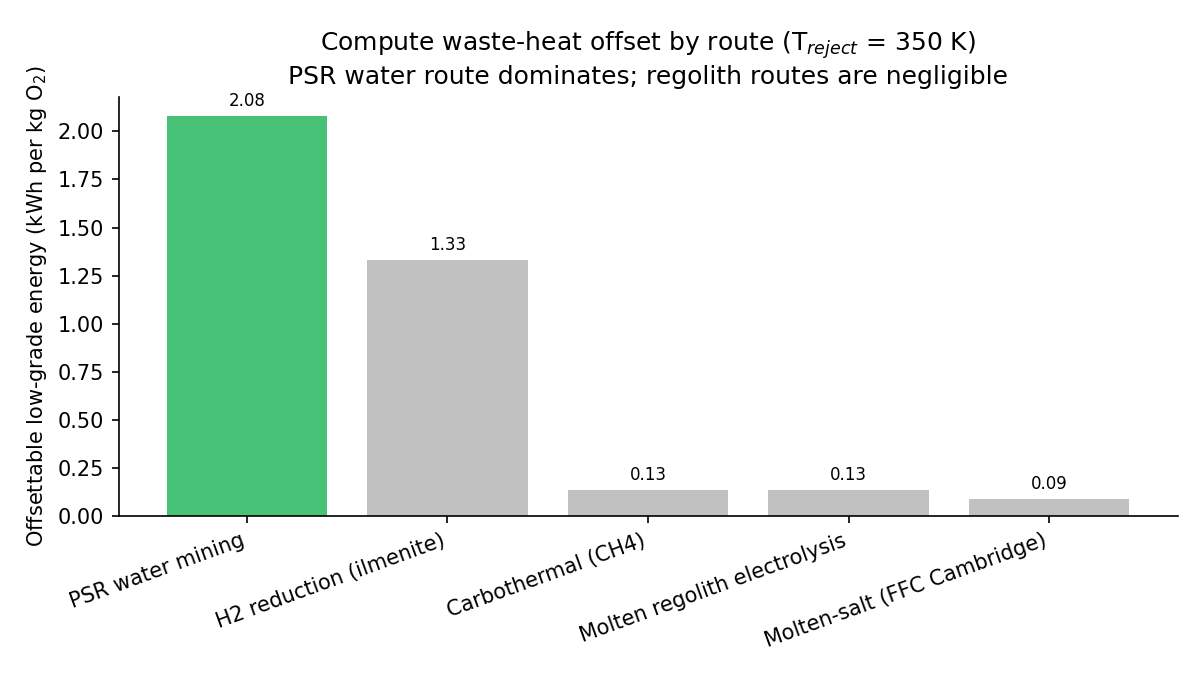
\includegraphics[width=0.85\textwidth]{../results/fig-waste-heat.png}
  \caption{Low-grade, waste-heat-offsettable energy per route ($T_{\mathrm{reject}}$ =
  350 K).}
  \label{fig:wasteheat}
\end{figure}

\begin{figure}[ht]
  \centering
  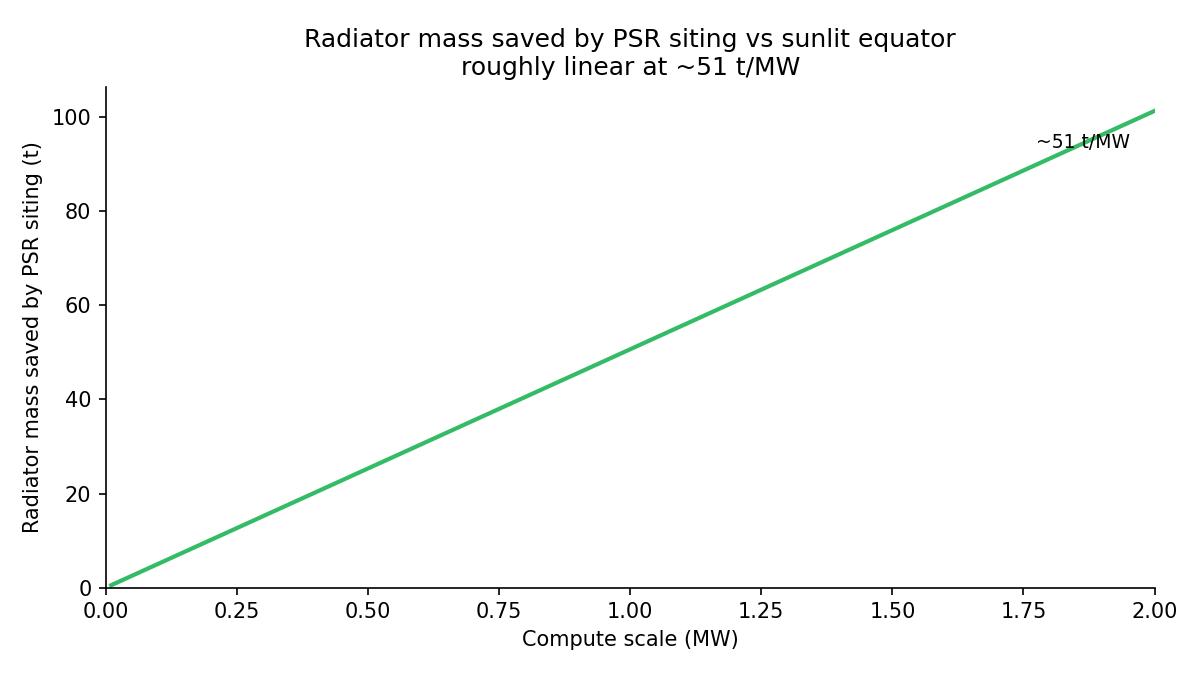
\includegraphics[width=0.85\textwidth]{../results/fig-radiator.png}
  \caption{Radiator mass saved by PSR siting vs a sunlit site (nominal $\sim$51 t/MW).}
  \label{fig:radiator}
\end{figure}

\section{Limitations}
\label{sec:limitations}

\begin{itemize}
  \item Steady-state production energy, power, and FSP landed mass only; capital cost,
    mobility, comms, site logistics, and demand are out of scope.
  \item Omitted energy terms are one-signed (they raise totals): standing radiative loss
    from continuously hot reactors (worst for the hottest route, MRE),
    comminution/beneficiation, electrolyzer heat-rejection parasitics, and, for the
    water route, months-long LH$_2$ zero-boil-off and power delivery into permanent
    shadow. Absolute kWh/kg figures are best read as lower bounds; the ranking is more
    robust than the levels.
  \item Three of five routes lack a direct independent electrical anchor.
  \item O$_2$ yield and reaction temperature are sampled independently (a residual
    idealization).
  \item Site geography and solar-thermal process heat are not modeled.
\end{itemize}

\section{Reproducibility}

\begin{verbatim}
pip install -e .
python -m lpem                 # Table 1
python -m lpem --dominance     # Table 2
python -m lpem --sensitivity mre   # Section 5 tornado
python -m lpem --plant-tonnes 50   # Section 7
python -m lpem --waste-heat --benefit   # Section 8
python scripts/make_figures.py     # Figures 1-3
pytest                         # 48 tests, incl. the validation anchors
\end{verbatim}

\section*{References}

The full bibliography (with DOIs/URLs) is in \texttt{paper/REFERENCES.md} and
\texttt{paper/references.bib}. Key sources: \citet{leger2025} (PNAS);
\citet{taylor1993}; \citet{carr1963}; \citet{allanore2015} (J. Electrochem. Soc.);
\citet{schreiner2016sizing} (Adv. Space Res.); \citet{kornuta2019} (REACH);
\citet{hauch2020} (Science); \citet{colaprete2010} (Science).

\bibliographystyle{plainnat}
\bibliography{references}

\end{document}
